\subsection{Differential gears} \label{sec:Differentialgears}

The differential gear box is located as the first component in the drivetrain, after the connection to the motor (Part 2 on \figref{vehicleDescriptionDriveTrain} in \secref{sec:Vehicledescription}).
When the servo is braking on one of the sides of the drivetrain, the differential gears transfer the rotational energy from this side to the other side. This minimize the lose of energy when braking. The extra speed, sent to the other belt that is not braking, will make the vehicle turn faster compared to a simple brake.

A differential gear system can be seen on \figref{diffGearLight}.

\begin{figure}[H]
	\centering
	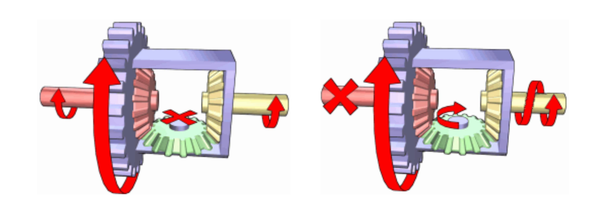
\includegraphics[scale=0.7]{figures/diffGearLight}
	\caption{Illustration of a differential gear system. On the left, the resistance on each side is equal, so the spider gear does not rotates. On the right, the resistance on the left side is bigger than the one on the right side, so the spider gear rotates and transfer more rotational energy to the right side. \cite{MechanicalEngineering}}
	\label{diffGearLight}
\end{figure}

The differential gear system contains a ring gear (blue), a spider gear (green), two side gears connected to the rest of the system (red and yellow) and a pinion gear (not shown on picture) connected to the ring gear, that transfer the power from the motor to the system.\\

When the motor is running, the pinion gear transfer a rotational energy to the ring gear. The spider gear, fixed on to the ring gear, begins to rotate around the side gear. If the resistance on both side gears is the same, the same power is needed to rotate the gears. Therefore the spider gear will not rotate around its own axis and apply the same rotational energy to each side gear.\\

When the resistance on both sides is not the same, i.g. if one of the side is being brake on, the spider gear will rotate around is own axis. There is a bigger resistance on one side than on the other, so the side not braking will be easier to rotate. The ring gear and the spider gear are rotating at the same speed around the two side gears, but the spider gear will apply less rotational energy on the braking side than on the other side, because of it own rotation. In the case that the resistance on one side is infinite, as the spider gear is rotating at the same speed that the ring gear, the side gear on the none braking side will therefore rotate twice as fast, with the assumption that there is no loss in the system.\\

For the differential gear system on the vehicle, there is a more complete setup, shown on \figref{diffGearFull}
	%\caption{Illustration of the differential gear system on the vehicle \cite{MechanicalEngineering}}

\begin{minipage}{\linewidth}
      \centering
      \begin{minipage}{0.65\linewidth}
          \begin{figure}[H]
              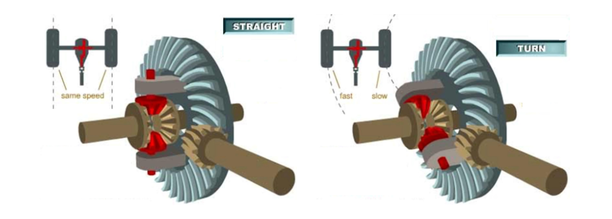
\includegraphics[width=0.95\textwidth]{figures/diffGearFull}
              \caption{Illustration of the differential gear system on the vehicle \cite{MechanicalEngineering}}
              \label{diffGearFull}
          \end{figure}
      \end{minipage}
      \hspace{0.05\linewidth}
      \begin{minipage}{0.25\linewidth}
      		\begin{enumerate}
      			\item Pinion gear
      			\item Ring gear
      			\item Spider gears
      			\item Side gears
      		\end{enumerate}
      \end{minipage}
  \end{minipage}




%\begin{table} [H]
%\begin{tabular}{p{3cm} p{3cm}}

%\begin{figure}
%	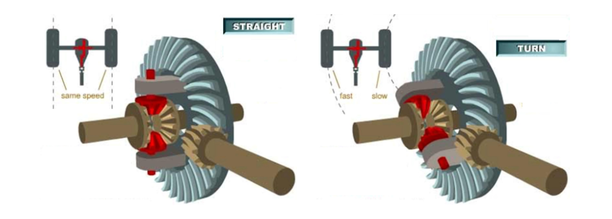
\includegraphics[scale=0.7]{figures/diffGearFull}
%	\label{diffGearFull}
%\end{figure}

%&

%\begin{enumerate}
 % \item Hallo
%\end{enumerate}

%\end{tabular}
%\end{table}




%\begin{figure} [h]
%	\centering
%	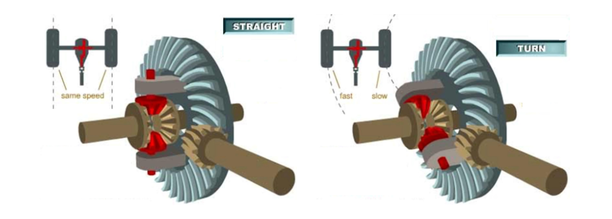
\includegraphics[scale=0.7]{figures/diffGearFull}
%	\caption{Illustration of the differential gear system on the vehicle \cite{MechanicalEngineering}}
%	\label{diffGearFull}
%\end{figure}

Instead of only having one spider gear (the green gear on \figref{diffGearLight}) there is two for more reliability and solidity, shown in red on \figref{diffGearFull}. The system works in the same way as with one spider gear, with the pinion gear (1) transfering the power to the ring gear (2). The spider gears (3) fixed on the ring gear rotates the side gears (4) compared to their own resistance.

Now that the vehicle has been presented and its limits analysed, the prototype contraints can be considered to aim the functionnalities needed in this project.

\subsection{Things that maybe should be placed in this section}

When a permanent magnet DC motor is used, the inductor and resistor in the motor causes a time constant, that the PWM time period should be less than:

\begin{flalign}
T &< 2 \cdot \frac{L_a}{R_a} \cdot ln(1-\frac{P}{100})\unit{s}
\end{flalign}

Where P is the duty cycle in percent, and La is the inductance in the motor, and Ra is the resistance in the motor.
